\section{Group Constant Data Generation on OpenMC}

The group constants required by either or both neutron diffusion and $S_N$ neutron transport
methods are:
%
\begin{itemize}
  \item $\Sigma_{t,g}$: Macroscopic total cross section in group $g$,
  \item $\Sigma_{r,g}$: Macroscopic removal cross section in group $g$,
  \item $\Sigma_s^{g'\rightarrow g}$: Macroscopic group-to-group scattering cross section matrix,
  \item $\Sigma_{s,l}^{g'\rightarrow g}$: $l$-th Legendre moment of the macroscopic
    group-to-group scattering cross section matrix,
  \item $\Sigma_{sp,l}^{g'\rightarrow g}$: $l$-th Legendre moment of the macroscopic
    group-to-group scattering production cross section matrix,
  \item $D_g$: $P_1$-based diffusion coefficient in group $g$,
  \item $\nu\Sigma_{f,g}$: Product of the average number of neutrons produced per fission and the
    macroscopic fission cross section in group $g$,
  \item $\chi_g$: Neutron fission spectrum in group $g$.
\end{itemize}
%
I generated the group constants using OpenMC's multigroup cross section generation capability
\cite{boyd_multigroup_2019}. The group constant postprocessing script for Moltres
(\texttt{moltres\_xs.py}) calculates $\Sigma_{r,g}$ as
%
\begin{align}
  \Sigma_{r,g} =& \sum^G_{g'\neq g}\Sigma_s^{g\rightarrow g'}+\Sigma_{a,g}-\left(\Sigma_{sp}^{g
    \rightarrow g} - \Sigma_s^{g\rightarrow g}\right)
  \shortintertext{where}
      \Sigma_{a,g} =& \mbox{ macroscopic absorption cross section in group $g$,} \nonumber \\
      \Sigma_{sp}^{g\rightarrow g} =& \mbox{ macroscopic scattering production cross section from
      group $g$ to $g$.} \nonumber
\end{align}
%
$\Sigma_{r,g}$ primarily represents the loss of neutrons from group $g$ through outscattering and
absorption. $\Sigma_{sp}^{g\rightarrow g}$ incorporates neutron multiplication effects from neutron
knockout reactions into the scattering cross section. Neutron knockout reactions are commonly
tallied as scattering reactions, but $\Sigma_{r,g}$ is a convenient parameter in which to
incorporate neutron knockout effects in the neutron diffusion equations. I ran all test cases for
$S_N$ and hybrid method calculations with up to the 2nd Legendre moments of the scattering
cross sections ($L=2$).

OpenMC uses the $P_1$ flux-limited formulation \cite{pomraning_flux-limited_1984} for calculating
$D_g$ as follows
%
\begin{align}
  D_g =& \frac{1}{3\Sigma_{tr,g}},
  \shortintertext{where}
  \Sigma_{tr,g} =& \frac{\langle\Sigma_{t,g}\phi_g\rangle-\langle\Sigma_{s1,g}\phi_g\rangle}
  {\langle\phi_g\rangle}, \nonumber \\
  \langle\Sigma_{t,g}\phi_g\rangle =& \int_{r\in V}dr \int_{4\pi}d\Omega\int^{E_{g-1}}_{E_g}dE\
  \Sigma_{t,g}(r,E)\Psi(r,E,\Omega), \nonumber \\
  \langle\Sigma_{s1,g}\phi_g\rangle =& \int_{r\in V}dr \int_{4\pi}d\Omega\int^{E_{g-1}}_{E_g}dE
  \int_{4\pi}d\Omega'\int^{\infty}_0dE'\int^1_{-1}d\mu\ \mu\Sigma_s(r,E'\rightarrow E,\Omega'\cdot
  \Omega)\phi(r,E',\Omega'), \nonumber \\
  \langle \phi \rangle =& \int_{r\in V}dr\int_{4\pi}d\Omega\int^{E_{g-1}}_{E_g}dE\ \Psi(r,E,\Omega)
  .\nonumber
\end{align}

I ran all \gls{MSRE} neutronics simulations with the eight neutron energy group structure proposed
by Jaradat for \gls{MSRE} analysis \cite{jaradat_development_2021-1}.
Table \ref{table:energy-group} shows the upper neutron energy bounds of the eight-group structure.
I selected this energy group structure as a compromise between accuracy and computational expense
among the various group structures investigated by Jaradat ranging from four to sixteen groups.

\begin{table}[htb]
  \centering
  \caption{Neutron energy group structure in this work. Originally devised by Jaradat
  \cite{jaradat_development_2021-1}.}
  \begin{tabular}{c S}
    \toprule
    Group & {Upper energy bound [eV]} \\
    \midrule
    1 & 2.000$\times 10^7$ \\
    2 & 1.353$\times 10^6$ \\
    3 & 6.734$\times 10^4$ \\
    4 & 9.118$\times 10^3$ \\
    5 & 1.487$\times 10^2$ \\
    6 & 4.000$\times 10^0$ \\
    7 & 6.250$\times 10^{-1}$ \\
    8 & 8.000$\times 10^{-2}$ \\
    \bottomrule
  \end{tabular}
  \label{table:energy-group}
\end{table}

I ran all cases on OpenMC to generate the required group constants and reference $k_\text{eff}$
values to assess the accuracy of the deterministic methods against OpenMC in continuous-energy
(OpenMC-CE) and multigroup (OpenMC-MG) modes. Table \ref{table:var} shows how the
position, direction of travel, neutron energy, and angle-dependence in $\Sigma_s$ are represented
by OpenMC and the deterministic methods. The hybrid $S_N$-diffusion method features representations
from either $S_N$ or neutron diffusion depending on the subregion under consideration.
Comparing OpenMC-MG results with OpenMC-CE results allows us
to quantify errors arising from neutron energy group discretization and the scattering cross
section simplifications.

\begin{table}[tb!]
  \centering
  \footnotesize
  \caption{Variable representations in OpenMC under continuous-energy (OpenMC-CE) and multigroup
  (OpenMC-MG) modes, and in the $S_N$ neutron transport and neutron diffusion.}
  \begin{tabular}{c c c c c c}
    \toprule
    Variable & OpenMC-CE & OpenMC-MG & $S_N$ Transport & Diffusion \\
    \midrule
    Position, $\bm{r}$ & Continuous & Continuous & Discrete & Discrete \\
    Direction of travel, $\bm{\hat{\Omega}}$ & Continuous & Continuous & Discrete & N/A \\
    Energy, $E$ & Continuous & Discrete & Discrete & Discrete & Discrete \\
    Angle-dependence in $\Sigma_s$ & Continuous & $L=2$ & $L=2$
    & N/A \\
    \bottomrule
  \end{tabular}
  \label{table:var}
\end{table}

\section{1-D Models}

\subsection{1-D Model Setup}

\subsubsection{Model Geometry}

I designed six 1-D test cases with increasing complexity to verify the $S_N$ and hybrid
$S_N$-diffusion implementations and to test the performance of the hybrid
method in response to various geometrical features. The last two cases resemble the
reference \gls{MSRE} design \cite{robertson_msre_1965}, which has centrally located control rods
and air-filled rod guide tubes. Figure \ref{fig:case-geom} shows the geometries of Cases 1a to
3b. All geometries have reflective boundary conditions at $x=0$ cm to reduce computational costs by
creating half-core or repeating unit cell models. Cases 1a and 1b are repeating unit
cell models with reflecting boundaries on the right-side boundaries. Cases 2a, 2b, 3a, and 3b
are 1-D half-core models with vacuum boundaries on the right-side boundaries.

Cases 1a and 1b are simple test cases containing neutron multiplying regions. Cases 1a and 1b serve
to verify basic neutronics phenomena modeling (e.g., fission, scattering, absorption) of the newly
implemented $S_N$ and neutron diffusion methods in Python and $S_N$ method in Moltres. I did not
apply the hybrid method on these cases. Cases 2a and 2b represent 1-D models of the \gls{MSRE} with
air-filled control rod guide tube regions, a homogenized fuel-graphite lattice regions, and outer
vessel regions. Case 2b additionally contains a 0.5cm-thick control rod region to contrast with
Case 2a for control rod worth calculations. Cases 3a and 3b retain the heterogeneous fuel-graphite
lattice geometry present in the \gls{MSRE}.

\begin{figure}[htb!]
  \centering
  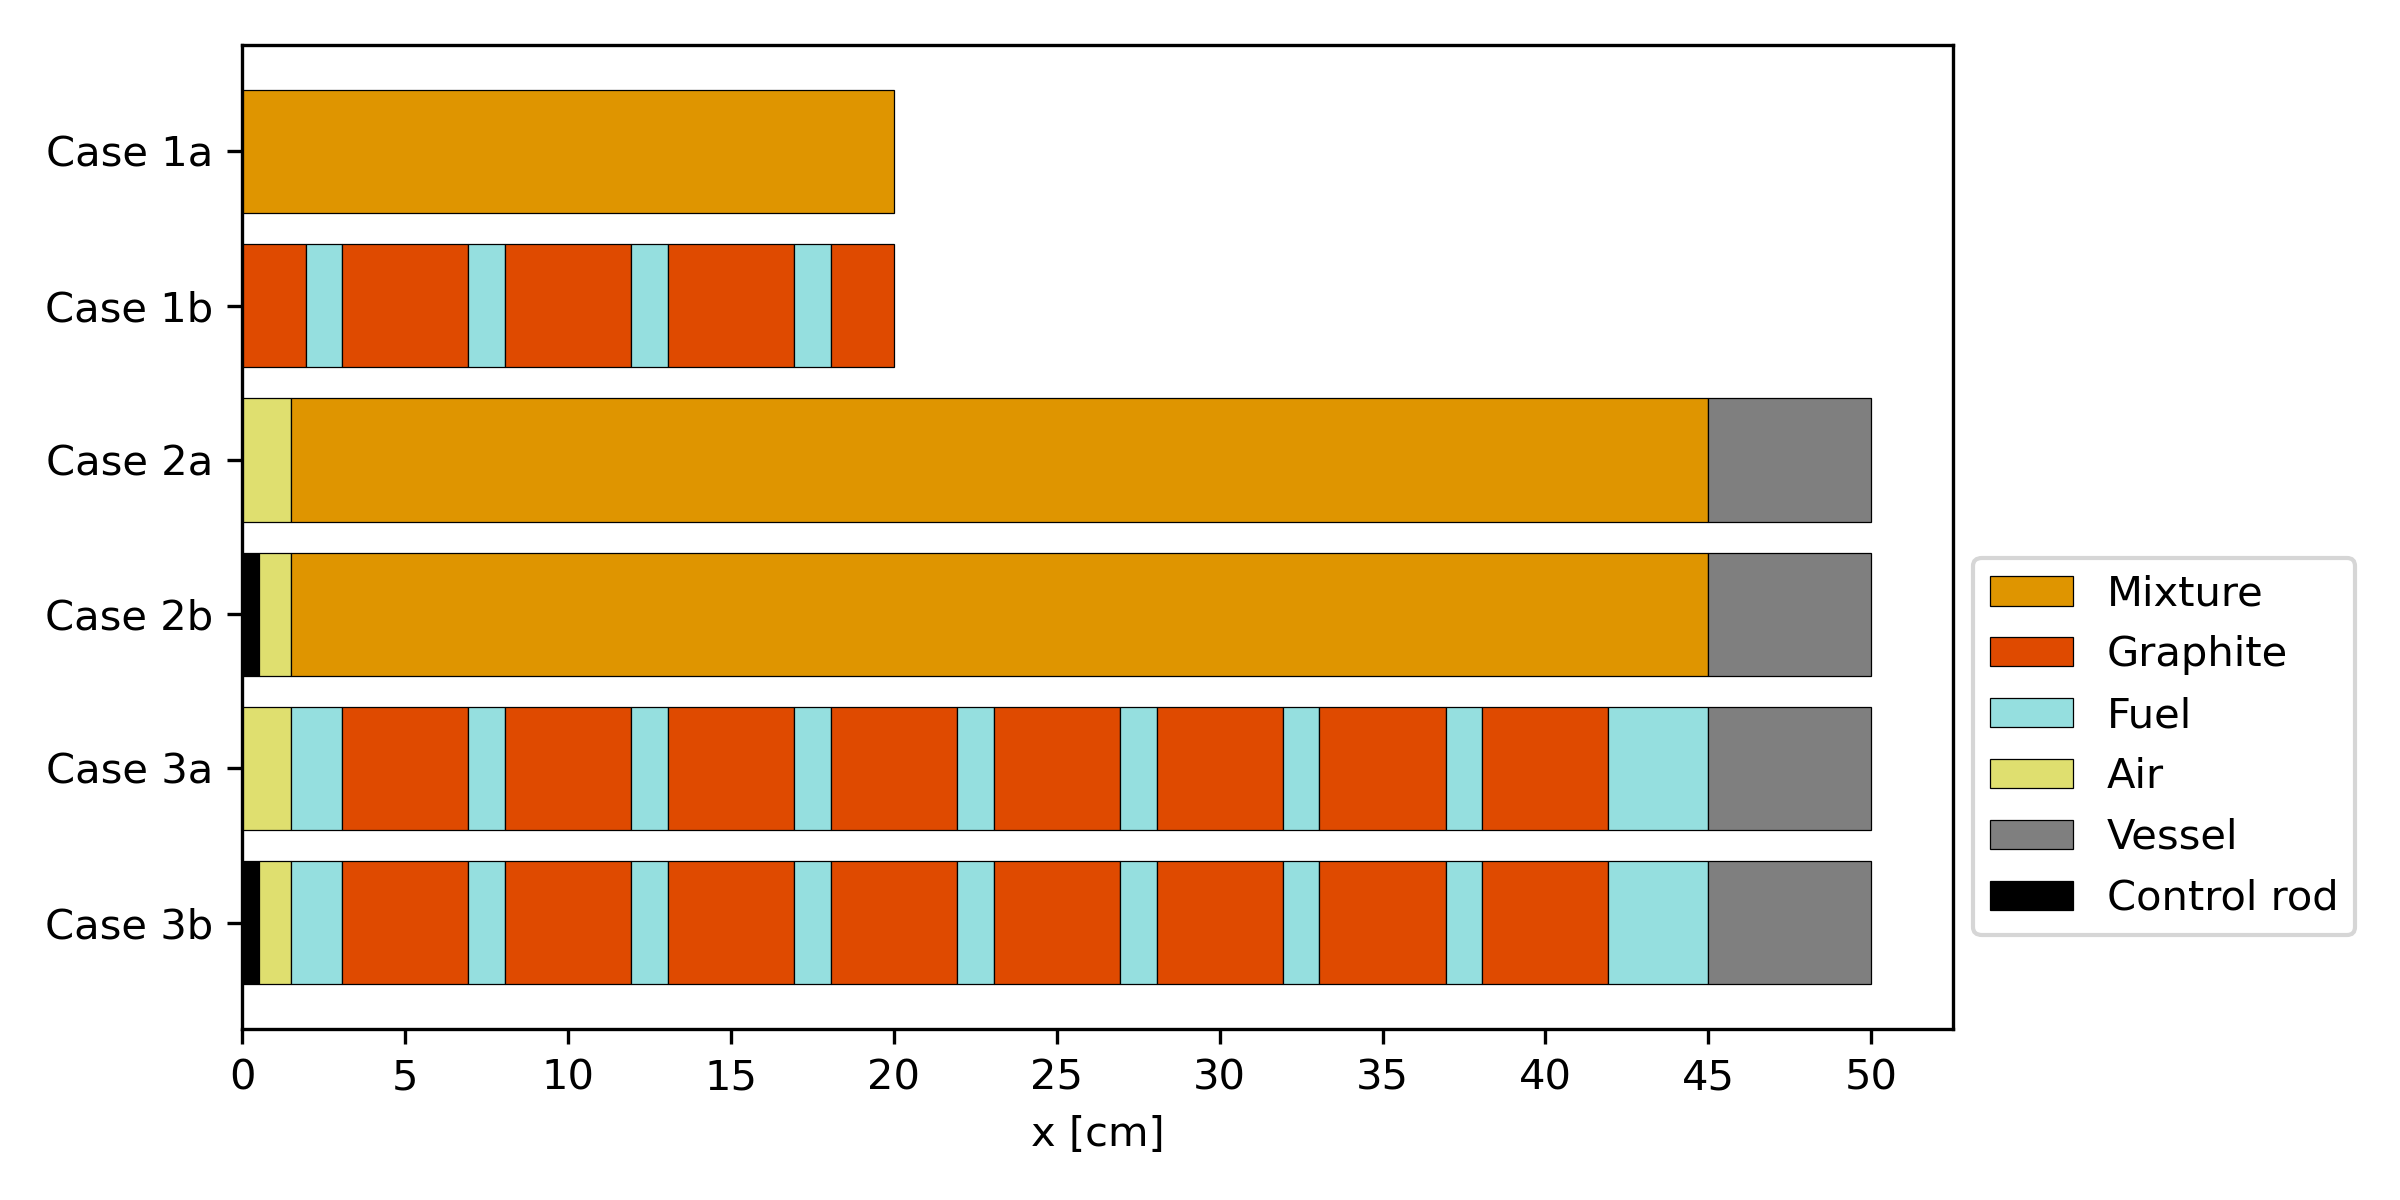
\includegraphics[width=\columnwidth]{case-geometry}
  \caption{Geometries of the 1-D test cases. The material labeled ``mixture'' represents a
    homogeneous mixture of fuel and graphite at a ratio of 22.5\%-77.5\% by volume. All geometries
    have reflective boundary conditions on the boundary at $x=0$ cm. The right-side boundaries are
    reflective for Cases 1a and 1b, and vacuum for Cases 2a, 2b, 3a, and 3b.}
  \label{fig:case-geom}
\end{figure}

\subsubsection{Mesh Convergence Tests}

\begin{figure}[htb!]
  \centering
  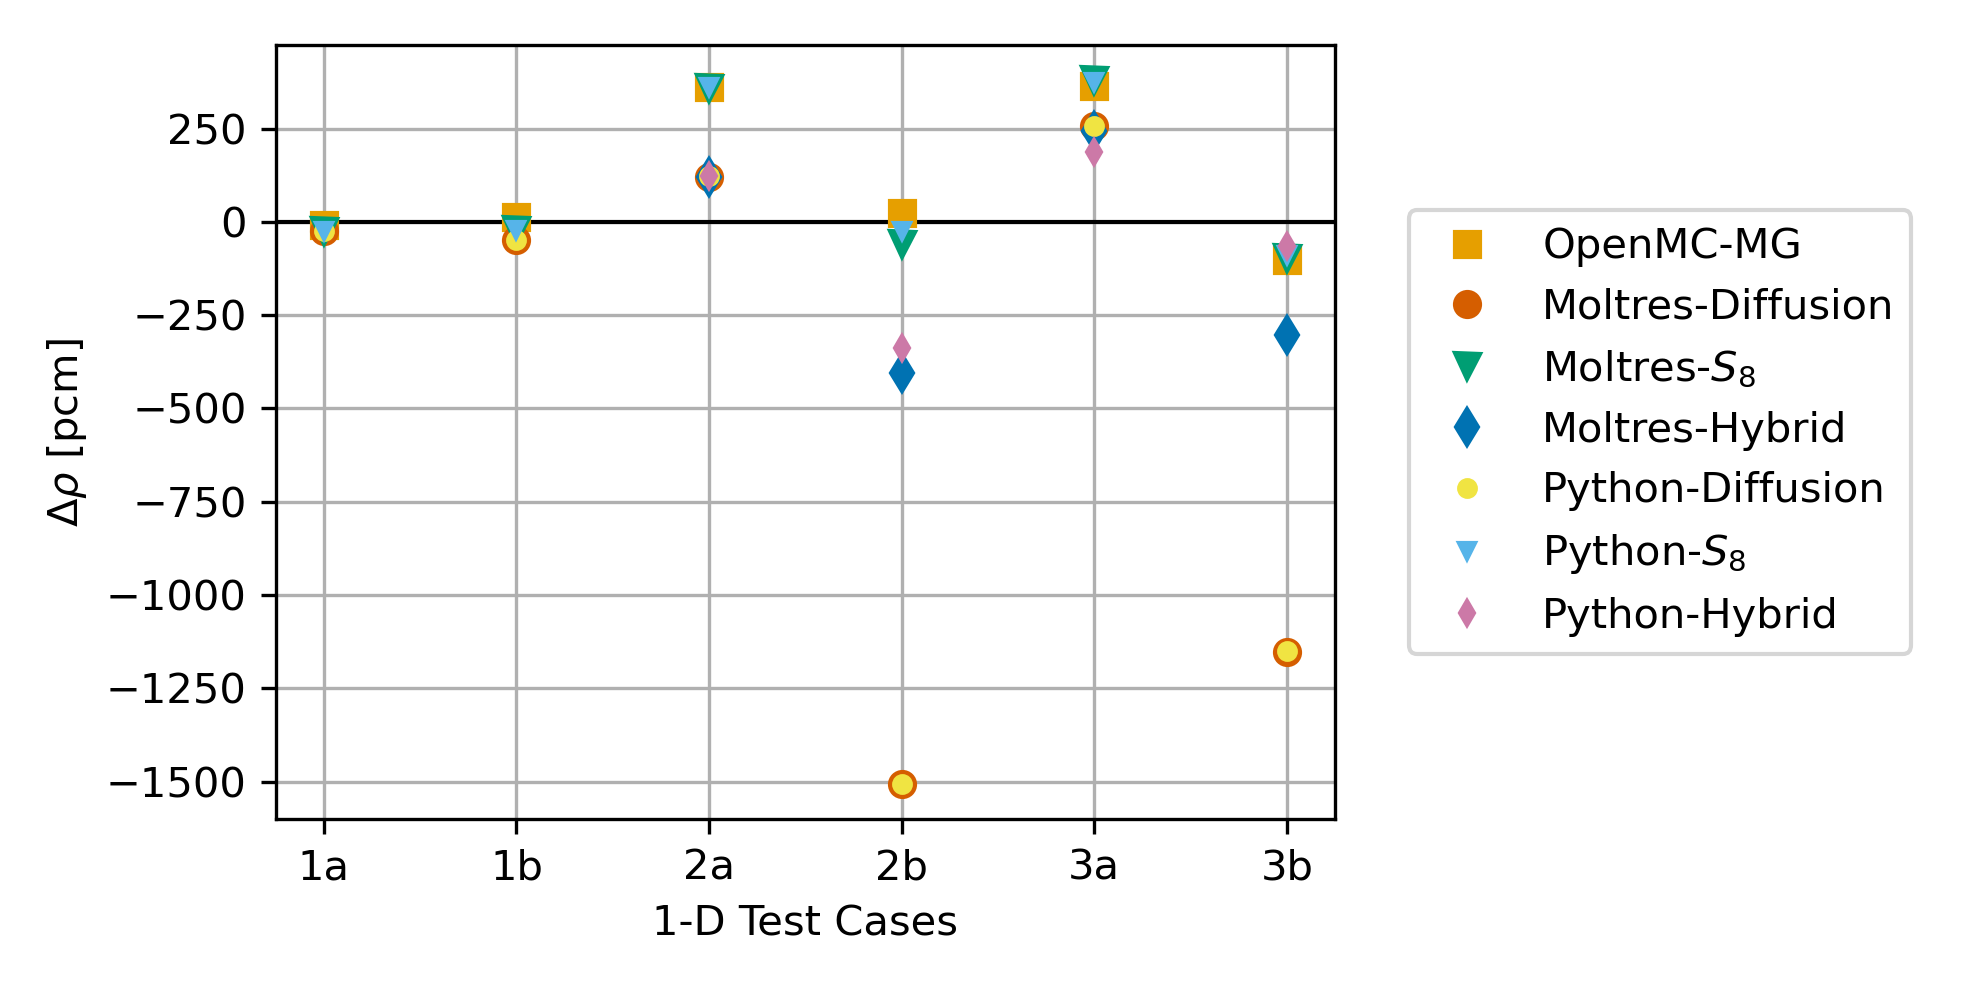
\includegraphics[width=\columnwidth]{rho}
  \caption{}
  \label{fig:1d-rho}
\end{figure}

\begin{figure}[htb!]
  \centering
  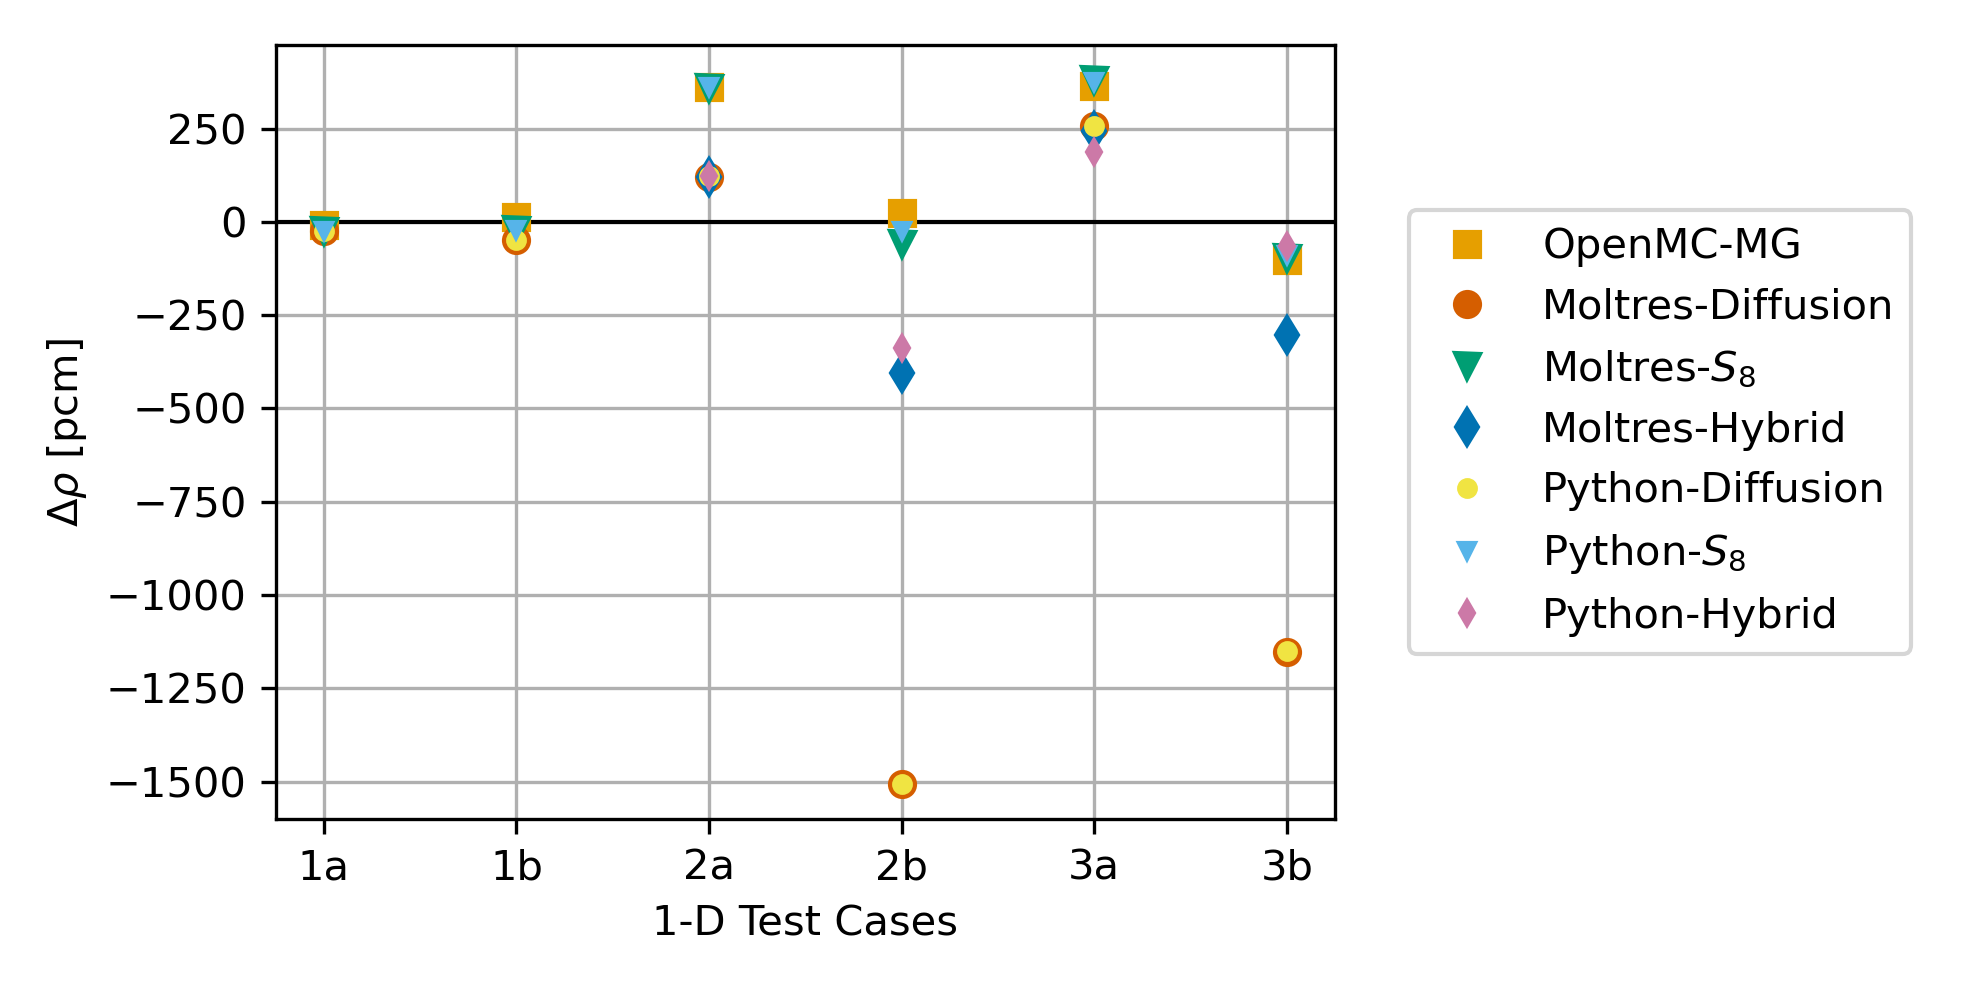
\includegraphics[width=\columnwidth]{rho}
  \caption{}
  \label{fig:1d-rho}
\end{figure}

\subsection{1-D Numerical Results}

\begin{figure}[htb!]
  \centering
  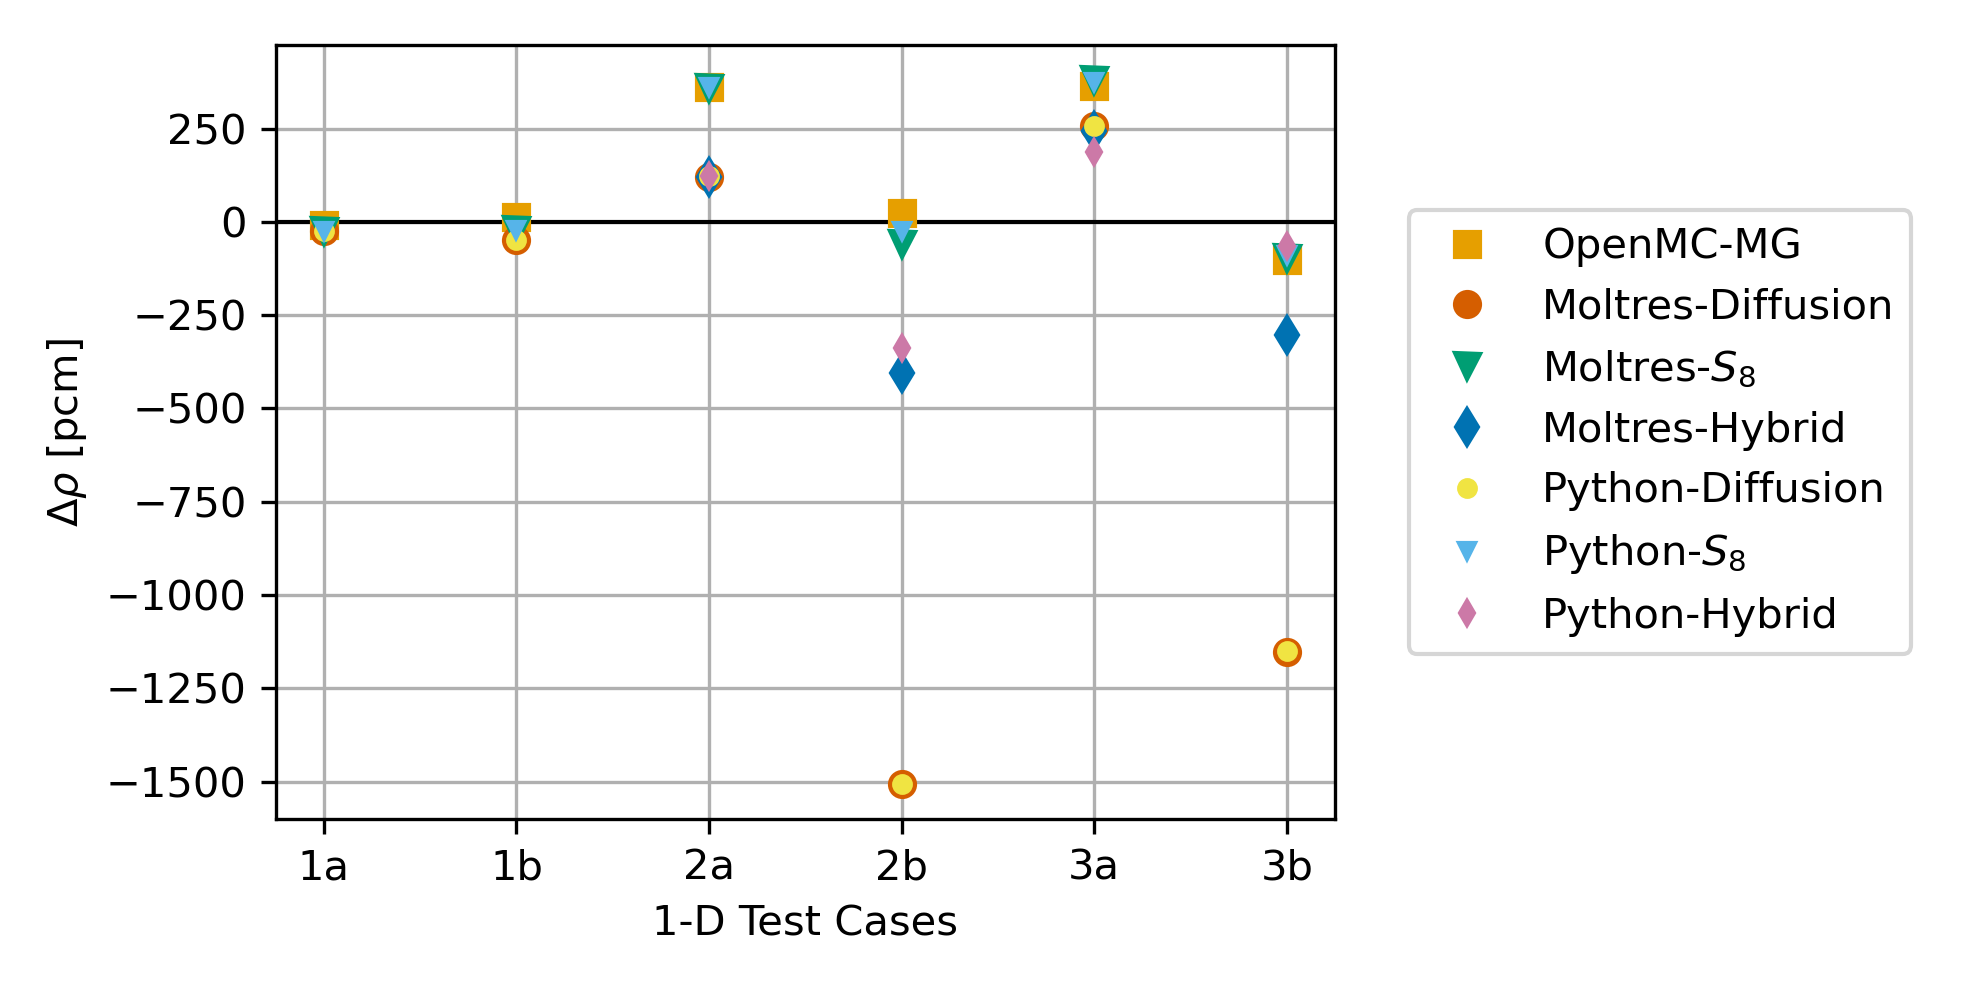
\includegraphics[width=\columnwidth]{rho}
  \caption{}
  \label{fig:1d-rho}
\end{figure}

\begin{figure}[htb!]
  \centering
  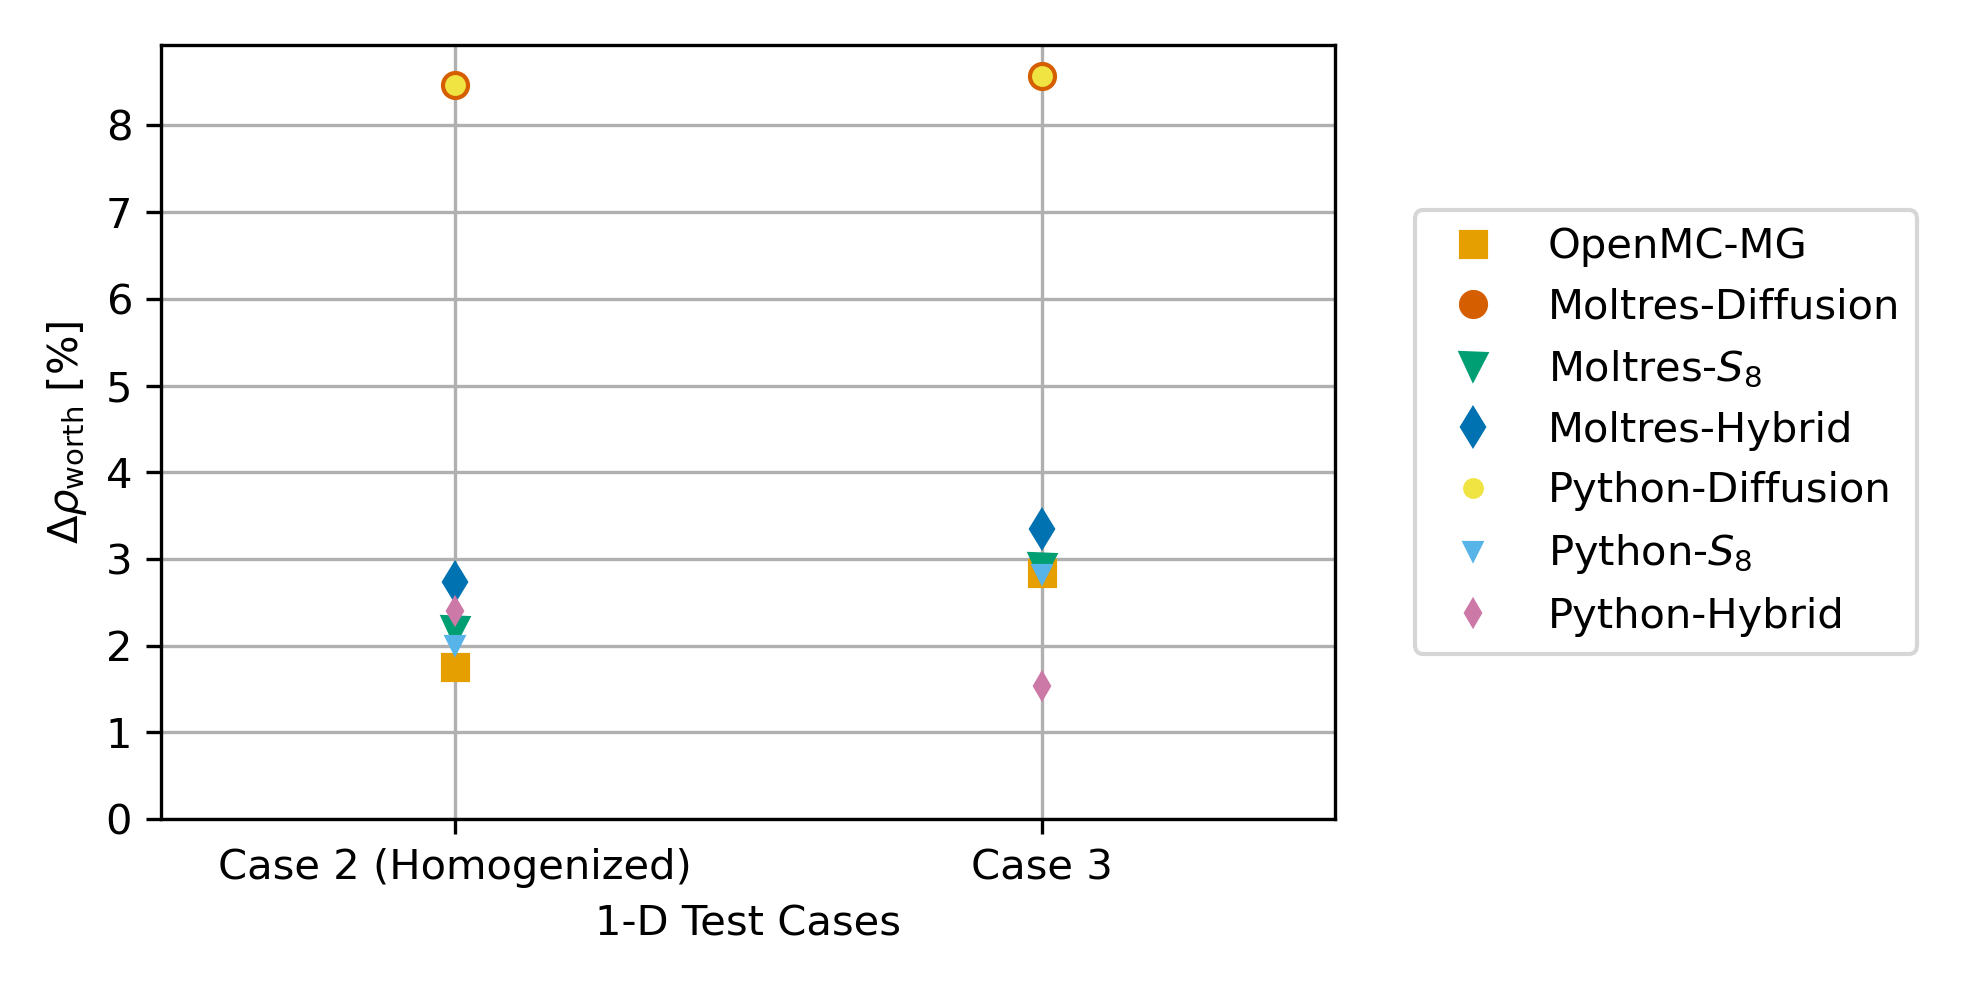
\includegraphics[width=\columnwidth]{worth}
  \caption{}
  \label{fig:1d-worth}
\end{figure}

\section{2-D Models}

\subsection{2-D Model Setup}

\subsection{2-D Numerical Results}

\section{3-D Models}

\subsection{3-D Model Setup}

\subsection{3-D Numerical Results}
